\chapter{Contributions à l'indexation automatique par termes-clés}
\chaptermark{Contribution à l'indexation par termes-clés}
\label{chap:main-automatic_keyphrase_annotation}
  \chaptercite{
    We analysed [\dots] the upper-bound performance for [the keyphrase
    extraction] task, and demonstrated that there is still room for improvement
    over the task.
  }{
    \newcite{kim2010semeval}
  }

  \section{Introduction}
  \label{sec:main-automatic_keyphrase_annotation-introduction}
    \TODO{chaine de traitement classique}
    \TODO{Extraction Vs. Assignation => Libre Vs. Controllé}

  %-----------------------------------------------------------------------------

  \section{Sélection des termes-clés candidats}
  \label{sec:main-automatic_keyphrase_annotation-keyphrase_candidate_selection}
    \subsection{Analyse des propriétés linguistiques des termes-clés}
    \label{subsec:main-automatic_keyphrase_annotation-keyphrase_candidate_selection-analysis_of_keyphrase_properties}

    \subsection{Filtrage des modificateurs}
    \label{subsec:main-automatic_keyphrase_annotation-keyphrase_candidate_selection-modifiers_filtering}

    \subsection{Evaluation}
    \label{subsec:main-automatic_keyphrase_annotation-keyphrase_candidate_selection-evaluation}
      \subsubsection{Evaluation intrinsèque}
      \label{subsubsec:main-automatic_keyphrase_annotation-keyphrase_candidate_selection-evaluation-intrinsic_evaluation}

      \subsubsection{Evaluation extrinsèque}
      \label{subsubsec:main-automatic_keyphrase_annotation-keyphrase_candidate_selection-evaluation-extrinsic_evaluation}

  %-----------------------------------------------------------------------------

  \section{Extraction automatique non supervisée de termes-clés}
  \label{sec:main-automatic_keyphrase_annotation-unsupervised_automatic_keyphrase_extraction}
    \subsection{TopicRank}
    \label{subsec:main-automatic_keyphrase_annotation-unsupervised_automatic_keyphrase_extraction-topicrank}
      % Qu'est-ce que TopicRank ?
      TopicRank est une méthode non supervisée d'extraction de termes-clés qui
      modélise un document sous la forme d'un graphe de sujets.
      % Quels problèmes résout-il ?
      Elle se différencie des autres méthodes à base de graphe, car, plutôt que
      de chercher les mots importants du document, elle cherche ses sujets
      importants.
      % Quel en est le fonctionnement général ?
      Notre méthode repose sur les trois étapes suivantes qui seront détaillées
      dans la suite~: identification des sujets~; ordonnancement des sujets~;
      sélection des termes-clés.

      \subsubsection{Identification des sujets}
      \label{subsubsec:main-automatic_keyphrase_annotation-unsupervised_automatic_keyphrase_extraction-topicrank-topic_identification}
        Dans ce travail, un sujet est une information générale ou le plus
        souvent spécifique véhiculée par au moins une unité textuelle présente
        dans le document analysé. Nous ne nous reposons donc pas sur une
        formulation approfondie d'un sujet, nous groupons seulement les
        termes-clés candidats lorsque ceux-ci véhiculent la même information.

        % Que nous faut-il pour identifier les sujets ?
        La première étape de l'identification des sujets consiste à sélectionner
        les termes-clés candidats.
        % Quels candidats composent les sujets ?
        Afin de réaliser une identification de qualité des sujets, nous excluons
        la sélection des n-grammes qui fournit beaucoup plus de candidats non
        pertinents que les autres méthodes. Concernant le choix entre la
        sélection des \textit{chunks} nominaux et la sélection des plus longues
        séquences de noms et d'adjectifs, nous suivons
        \newcite{wan2008expandrank} et \newcite{hassan2010conundrums} en
        sélectionnant les plus longues séquences de noms et d'adjectifs. Cette
        méthode présente l'avantage de fournir des candidats grammaticalement
        corrects et de ne nécessiter qu'une adaptation limitée pour le
        traitement de documents d'une autre langue.

        % Comment détectons nous deux candidats appartenant au même sujet ?
        La seconde étape de l'identification des sujets consiste à grouper les
        termes-clés candidats lorsqu'ils appartiennent au même sujet. Dans le
        souci de proposer une méthode ne faisant pas l'usage de données
        supplémentaires, nous optons pour un groupement quelque peu naïf des
        candidats. Deux candidats $c_1$ et $c_2$ sont groupés en fonction d'une
        similarité de Jaccard par laquelle ils sont considérés comme des sacs de
        mots tronqués selon la méthode de racinisation\footnote{Cette
        racinisation a pour effet de grouper les candidats qui varient
        uniquement en termes de flexion ou de dérivation.} de
        \newcite{porter1980suffixstripping}~:
        \begin{align}
          \text{sim}(c_1, c_2) &= \frac{\|c_1 \cap c_2\|}{\|c_1 \cup c_2\|} \label{equa:jaccard}
        \end{align}
        Cette mesure est naïve dans le sens où l'ordre des mots, leur ambiguïté
        et les liens de synonymie ne sont pas pris en compte. À cela s'ajoute
        aussi des erreurs introduites par l'usage de la méthode de
        \newcite{porter1980suffixstripping} (par exemple les mots
        \og{}empire\fg{} et \og{}empirique\fg{} partagent le même radical,
        \og{}empir\fg{}).

        % Comment groupons nous les candidats d'un même sujet ?
        Une fois la similarité connue entre toutes les paires de candidats, nous
        appliquons l'algorithme de groupement hiérarchique agglomératif
        (\textit{Hierarchical Agglomerative Clustering -- HAC}). Initialement,
        chaque candidat représente un groupe et, jusqu'à l'obtention d'un nombre
        prédéfini de groupes, les deux groupes ayant la plus forte similarité
        sont unis pour ne former qu'un seul groupe. Afin de ne pas fixer le
        nombre de sujets à créer comme condition d'arrêt de l'algorithme, nous
        définissons un seuil de similarité $\zeta$ entre les groupes deux à
        deux. Cette similarité entre deux groupes est déterminée à partir de la
        similarité de Jaccard calculée entre les candidats de chaque groupe. Il
        existe trois stratégies pour calculer la similarité entre deux groupes~:
        \begin{itemize}
          \item{simple~: la plus grande valeur de similarité entre les candidats
                des deux groupes sert de similarité entre eux~;}
          \item{complète~: la plus petite valeur de similarité entre les
                candidats des deux groupes sert de similarité entre eux~;}
          \item{moyenne~: la moyenne de toutes les similarités entre les
                candidats des deux groupes sert de similarité entre eux
                (compromis entre les stratégies simple et complète).}
        \end{itemize}
        L'une ou l'autre de ces stratégies est à privilégier en fonction du type
        des candidats extraits. Pour des candidats qui ont de forts
        recouvrements, tels que les n-grammes, il semble plus pertinent
        d'utiliser la stratégie complète qui est la moins agglomérative. Dans le
        cas de TopicRank, où les candidats sont de meilleure qualité que les
        n-grammes, la stratégie moyenne est une meilleure alternative.

      \subsubsection{Ordonnancement des sujets}
      \label{subsubsec:main-automatic_keyphrase_annotation-unsupervised_automatic_keyphrase_extraction-topicrank-topic_ranking}
        % Quel est le but de l'ordonnancement ?
        % Comment est-il effectué ?
        L'ordonnancement des sujets a pour objectif de trouver quels sont ceux
        qui ont le plus d'importance dans le document analysé. À l'instar de
        \newcite{mihalcea2004textrank}, l'importance des sujets est déterminée à
        partir d'un graphe.

        % Comment le graphe est-il construit ?
        Les sujets du document analysé composent les n\oe{}uds $V$ du graphe
        complet $G = (V, E)$, où $E$ est l'ensemble des liens entre les
        n\oe{}uds\footnote{$E = \{(v_1, v_2)\ |\ \forall{v_1, v_2 \in V}, v_1
        \neq v_2\}$, car $G$ est un graphe complet.}. Du fait que le graphe
        utilisé soit un graphe complet, la pondération de ses arêtes est l'étape
        la plus importante pour rendre possible un ordonnancement efficace des
        sujets. Pour cette pondération, nous suivons \newcite{wan2008expandrank}
        et utilisons la force du lien sémantique entre les sujets. Cependant,
        parce que nous utilisons un graphe complet, il ne nous est pas possible
        de représenter cette force par le nombre de cooccurrences entre les
        sujets. Pour préserver l'intuition derrière l'usage du nombre de
        cooccurrences, nous représentons la force du lien sémantique entre deux
        sujets par la distance entre les candidats des sujets dans le document~:
        \begin{align}
          \text{poids}(s_i, s_j) &= \sum_{c_i \in s_i}\ \sum_{c_j \in s_j} \text{dist}(c_i, c_j) \label{math:ponderation}\\
          \text{dist}(c_i, c_j) &= \sum_{p_i \in \text{pos}(c_i)}\ \sum_{p_j \in \text{pos}(c_j)} \frac{1}{|p_i - p_j|} \label{math:distance}
        \end{align}
        où $\text{poids}(s_i, s_j)$ est le poids de l'arête entre les sujets
        $s_i$ et $s_j$, et où $\text{dist}(c_i, c_j)$ représente la force
        sémantique entre les candidats $c_i$ et $c_j$, calculée à partir de
        leurs positions respectives, $\text{pos}(c_i)$ et $\text{pos}(c_j)$,
        dans le document.

        % Comment le graphe est-il utilisé pour ordonner les sujets ?
        % Quelle est l'intuition de PageRank/TextRank ?
        Une fois le graphe construit, l'algorithme d'ordonnancement de TextRank
        est utilisé pour identifier quels sont les sujets les plus importants du
        document. Cet ordonnancement se fonde sur le principe de recommandation
        (de vote), c'est-à-dire un sujet est d'autant plus important s'il est
        fortement connecté avec un grand nombre de sujets et si les sujets avec
        lesquels il est fortement connecté sont importants~:
        \begin{align}
          \text{importance}(s_i) = (1 - \lambda) + \lambda \times \sum_{s_j \in V_i} \frac{\text{poids}(s_i, s_j) \times \text{importance}(s_j)}{\sum_{s_k \in V_j} \text{poids}(s_j, s_k)} \label{math:textrank}
        \end{align}
        où $V_i$ est l'ensemble des sujets connectés au sujet\footnote{$V_i =
        \{v_i\ |\ \forall{v_j \in V}, v_j \neq v_i\}$, car $G$ est un graphe
        complet.} $s_i$ et où $\lambda$ est un facteur d'atténuation définit à
        0,85 d'après les recommandations de \newcite{brin1998pagerank}.

      \subsubsection{Sélection des termes-clés}
      \label{subsubsec:main-automatic_keyphrase_annotation-unsupervised_automatic_keyphrase_extraction-topicrank-keyphrase_selection}
        % De quoi s'agit-il ?
        La sélection des termes-clés est la dernière étape de TopicRank. Elle
        consiste à chercher les termes-clés candidats qui représentent le mieux
        les sujets importants. Dans le but de ne pas extraire de termes-clés
        redondants, un seul candidat est sélectionné par sujet.
        % Quel en est le but ?
        Ainsi, pour $k$ sujets, $k$ termes-clés non redondants couvrant
        exactement $k$ sujets sont extraits.

        % Quelles sont les différentes stratégies envisageable ?
        La difficulté de ce principe de sélection réside dans la capacité à
        trouver parmi plusieurs termes-clés candidats d'un même sujet celui qui
        le représente le mieux. Nous proposons trois stratégies de sélection
        pouvant répondre à ce problème~:
        \begin{itemize}
          \item{la première position~: en supposant qu'un sujet est tout d'abord
                introduit sous sa forme la plus appropriée, le terme-clé
                candidat sélectionné pour un sujet est celui qui apparaît en
                premier dans le document analysé;}
          \item{la fréquence~: en supposant que la forme la plus représentative
                d'un sujet est sa forme la plus fréquente, le terme-clé candidat
                sélectionné pour un sujet est celui qui est le plus fréquent
                dans le document analysé;}
          \item{le centroïde~: le terme-clé candidat sélectionné pour un sujet
                est celui qui est le plus similaire aux autres candidats du
                sujet (voir l'équation~\ref{equa:jaccard}).}
        \end{itemize}
        % Laquelle des trois stratégies semble être la mieux ?
        Parmi ces trois stratégies, celle qui semble la plus appropriée est la
        stratégie qui se fonde sur la première position des termes-clés
        candidats. Sélectionner les candidats les plus fréquents risque de ne
        pas être une solution stable selon les types de documents, en
        particulier selon leur taille, tandis que sélectionner les centroïdes
        risque de ne pas fournir les termes-clés les plus précis.

    \subsection{Evaluation}
    \label{subsec:main-automatic_keyphrase_annotation-unsupervised_automatic_keyphrase_extraction-evaluation}
      Pour valider notre approche, nous réalisons une première série
      d'évaluations visant à déterminer la configuration optimale de TopicRank.
      Nous comparons  ensuite Topic\-Rank aux travaux précédents et analysons
      l'impact de chacune de nos contributions.
      
      \subsubsection{Méthodes de référence}
      \label{subsubsec:main-automatic_keyphrase_annotation-unsupervised_automatic_keyphrase_extraction-evaluation-baselines}
        % Comment les baselines sont-elles choisies ?
        Dans nos expérimentations, nous comparons TopicRank à trois autres
        méthodes non supervisées d'extraction automatique de termes-clés. Nous
        choisissons TextRank et SingleRank, les deux méthodes qui sont la
        fondation des méthodes à base de graphe, et la méthode de pondération
        TF-IDF. Cette dernière méthode consiste à extraire en tant que
        termes-clés les candidats dont les mots sont importants. Un mot est
        considéré important dans un document s'il y est fréquent (TF élevé) et
        s'il a une forte spécificité (IDF élevé) calculée à partir de toute une
        collection de documents\footnote{Dans ce travail, nous utilisons la
        collection dont est extrait le document.} de sorte que moins il y a de
        documents qui contiennent le mot, plus forte est sa spécificité. TF-IDF
        prenant en compte la totalité du corpus, il s'agit de montrer que
        TopicRank est capable d'extraire le contenu principal d'un document sans
        nécessiter de données supplémentaires et qu'il est donc applicable à des
        documents de tous types pour lesquels aucun travail de collecte
        préalable n'est nécessaire.

        % Quelles sont les particularités liées à notre implémentation ?
        Au même titre que TopicRank, nous proposons une implémentation des
        méthodes de référence disponible sur la plate-forme de développement
        collaboratif
        GitHub\footnote{\url{https://github.com/adrien-bougouin/KeyBench/tree/ijcnlp_2013}}.
        Dans un souci de comparaison, lorsque les méthodes de référence
        partagent le même comportement que TopicRank, celui-ci est réalisé par
        le même composant.

      \subsubsection{Collections de données}
      \label{subsubsec:main-automatic_keyphrase_annotation-unsupervised_automatic_keyphrase_extraction-evaluation-evaluation_data}
        Afin de suivre \newcite{hassan2010conundrums} qui soulignent
        l'importance d'évaluer une méthode avec des collections de données aux
        configurations différentes pour mieux observer et comprendre son
        comportement, les collections de données utilisées dans ce travail
        diffèrent en termes de langue, nature, taille des documents et types
        d'annotateurs (auteurs, lecteurs ou les deux).

        DUC~\cite{over2001duc} est une collection en anglais issue des données
        de la campagne d'évaluation DUC-2001 qui concerne les méthodes de résumé
        automatique. Elle ne contient donc originellement pas d'annotations en
        termes-clés. Cependant, les 308 articles journalistiques de la partie
        test de DUC-2001 ont été annotés par \newcite{wan2008expandrank}. Nous
        utilisons ces 308 documents pour comparer TopicRank avec les méthodes de
        référence.

        SemEval~\cite{kim2010semeval} est la collection en anglais fournie lors
        de la campagne d'évaluation SemEval-2010 pour la tâche d'extraction
        automatique de termes-clés. Cette collection contient 244 articles
        scientifiques (conférences et ateliers) issus de la bibliothèque
        numérique ACM. La collection est répartie en deux sous-ensembles~: un
        ensemble de 144 documents d'entraînement et un ensemble de 100 documents
        de test. Lors de nos expériences, nous utilisons les 100 documents de
        l'ensemble de test pour comparer TopicRank avec les méthodes de
        référence et les 144 documents d'entraînement pour paramétrer TopicRank
        et SingleRank. En ce qui concerne les termes-clés associés aux
        documents, ce sont les termes-clés des auteurs combinés aux termes-clés
        donnés par des étudiants.

        WikiNews\footnote{\url{https://github.com/adrien-bougouin/WikinewsKeyphraseCorpus}}
        est une collection de 100 articles journalistiques en français que nous
        avons extraits du site Web
        WikiNews\footnote{\url{http://fr.wikinews.org}} entre les mois de mai et
        de décembre 2012. Pour l'annotation en termes-clés, nous avons demandé à
        neuf étudiants de master en TAL d'extraire (librement) les termes-clés
        de 33 documents, de sorte que chaque document soit annoté par au moins
        trois étudiants. Nous utilisons les 100 documents de Wikinews pour
        comparer TopicRank avec les méthodes de référence.

        DEFT~\cite{paroubek2012deft} est la collection fournie lors de la
        campagne d'évaluation DEFT-2012 pour la tâche d'extraction automatique
        de termes-clés. Celle-ci contient 234 documents en français issus de
        quatre revues de sciences humaines et sociales. Elle est divisée en deux
        sous-ensembles~: un ensemble d'entraînement contenant 141 documents et
        un ensemble de test contenant 93 documents. Lors de nos expériences,
        nous utilisons les 93 documents de l'ensemble de test pour comparer
        TopicRank avec les méthodes de référence et les 141 documents
        d'entraînement pour paramétrer TopicRank et SingleRank. Dans cette
        collection, seuls les termes-clés des auteurs sont disponibles.

        Le tableau~\ref{tab:donnees_de_test} donne les statistiques extraites
        des ensembles de test des quatre collections de données présentées
        ci-dessus. Les données sont divisées en deux langues (anglais et
        français), avec pour chaque langue une collection de documents courts
        (articles journalistiques) et une collection de documents de plus grande
        taille (articles scientifiques). Il est aussi important de noter qu'en
        fonction du type d'annotateurs, le nombre de termes-clés associés varie,
        de même que le nombre de termes-clés n'apparaissant pas dans les
        documents.
        \begin{table}
          \centering
          \begin{tabular}{@{~}l@{~}|@{~}c@{~}|@{~}c@{~}|@{~}c@{~}|@{~}c@{~}}
            \hline
            \textbf{Statistique} & \textbf{DUC} & \textbf{SemEval} & \textbf{WikiNews} & \textbf{DEFT}\\
            \hline
            Langue & Anglais & Anglais & Français & Français\\
            \hline
            Nature & Journalistique & Scientifique & Journalistique & Scientifique\\
            \hline
            \multirow{3}{*}[.35em]{Annotateurs} & \multirow{3}{*}[.35em]{Lecteurs} & Auteurs & \multirow{3}{*}[.35em]{Lecteurs} & \multirow{3}{*}[.35em]{Auteurs}\\
            \addlinespace[-.7\defaultaddspace]
            & & \& & &\\
            \addlinespace[-.7\defaultaddspace]
            & & Lecteurs & &\\
            \hline
            Documents & 308 & 100 & 100 & 93\\
            Mots/document & 900,7 & 5~177,7 & 308,5 & 6~839,4\\
            Termes-clés/document & 8,1 & 14,7 & 9,6 & 5,2\\
            Mots/termes-clés & 2,1 & 2,1 & 1,7 & 1,6\\
            \hline
            %Termes-clés manquants & 3,5\% & 22,1\% & 7,6\% & 21,1\% \\
            Termes-clés extractibles & 96,5~\% & 77,9~\% & 92,4~\% & 78,9~\% \\
            \hline
          \end{tabular}
          \caption{Statistiques sur les données de test utilisées. Les termes-clés
                   extractibles sont les termes-clés qui peuvent être extraits à
                   partir du contenu des documents.
                   \label{tab:donnees_de_test}}
        \end{table}

      \subsubsection{Prétraitement}
      \label{subsubsec:main-automatic_keyphrase_annotation-unsupervised_automatic_keyphrase_extraction-evaluation-preprocessing}
        Chaque document des collections de données utilisées subit les mêmes
        prétraitements. Chaque document est tout d'abord segmenté en phrases,
        puis en mots et enfin étiqueté grammaticalement. La segmentation en mots
        est effectuée par le TreeBankWordTokenizer, disponible avec la librairie
        python NLTK~\cite[\textit{Natural Language ToolKit}]{bird2009nltk}, pour
        l'anglais et par l'outil Bonsai, du Bonsai PCFG-LA
        parser\footnote{\url{http://alpage.inria.fr/statgram/frdep/fr_stat_dep_parsing.html}},
        pour le français. Quant à l'étiquetage grammatical, il est réalisé avec
        le Stanford POS tagger~\cite{toutanova2003stanfordpostagger} pour
        l'anglais et avec l'outil MElt~\cite{denis2009melt} pour le français.
        Tous ces outils sont utilisés avec leur configuration par défaut.

      \subsubsection{Mesures d'évaluation}
      \label{subsubsec:main-automatic_keyphrase_annotation-unsupervised_automatic_keyphrase_extraction-evaluation-evaluation_measures}
        Les performances des méthodes d'extraction de termes-clés sont exprimées
        en termes de précision (P), rappel (R) et f-score (f1-mesure, F). En
        accord avec l'évaluation menée dans les travaux précédents, nous
        considérons correcte l'extraction d'une variante flexionnelle d'un
        terme-clé de référence~\cite{kim2010semeval}. Les opérations de
        comparaison entre les termes-clés de référence et les termes-clés
        extraits sont donc effectuées à partir de la racine des mots qui les
        composent en utilisant la méthode de racinisation de
        \newcite{porter1980suffixstripping}.

      \subsubsection{Analyse empirique de TopicRank}
      \label{subsubsec:main-automatic_keyphrase_annotation-unsupervised_automatic_keyphrase_extraction-evaluation-empirical_analysis_of_topicrank}
        Dans cette section, nous effectuons des expériences préliminaires afin
        de déterminer quelle est la configuration optimale de TopicRank. En
        utilisant les ensembles d'entraînement de SemEval et de DEFT, nous
        réalisons deux expériences durant lesquelles nous faisons varier, dans
        un premier temps, le seuil de similarité ($\zeta$) et la stratégie de
        groupement (simple, complète et moyenne), puis dans un second temps, la
        stratégie de sélection du terme-clé candidat le plus représentatif de
        chacun des sujets les plus importants.
        \begin{figure}
          \centering
          \subfigure[SemEval]{
            \begin{tikzpicture}
              \pgfkeys{/pgf/number format/.cd, use comma, fixed}
              \begin{axis}[axis lines=middle,
                           x=0.37\linewidth,
                           xtick={0.0, 0.2, ..., 1.2},
                           xmin=0.0,
                           xmax=1.05,
                           xlabel=$\zeta$,
                           x label style={anchor=west},
                           y=0.012\textheight,
                           ytick={0, 5, 10, 15},
                           ymin=0,
                           ymax=18,
                           ylabel=F,
                           y label style={anchor=south}]
                % simple
                \addplot[green!66, mark=x] coordinates{
                  (0.05, 4.2)
                  (0.10, 4.2)
                  (0.15, 4.4)
                  (0.20, 4.7)
                  (0.25, 4.9)
                  (0.30, 5.3)
                  (0.35, 7.4)
                  (0.40, 7.4)
                  (0.45, 7.3)
                  (0.50, 7.3)
                  (0.55, 7.5)
                  (0.60, 7.5)
                  (0.65, 7.5)
                  (0.70, 8.0)
                  (0.75, 8.0)
                  (0.80, 8.0)
                  (0.85, 8.0)
                  (0.90, 8.0)
                  (0.95, 8.0)
                  (1.00, 8.0)
                };
                % complet
                \addplot[cyan!66, mark=+] coordinates{
                  (0.05, 11.5)
                  (0.10, 11.5)
                  (0.15, 10.9)
                  (0.20, 10.3)
                  (0.25, 9.3)
                  (0.30, 7.8)
                  (0.35, 7.6)
                  (0.40, 7.6)
                  (0.45, 7.5)
                  (0.50, 7.5)
                  (0.55, 7.5)
                  (0.60, 7.5)
                  (0.65, 7.6)
                  (0.70, 8.0)
                  (0.75, 8.0)
                  (0.80, 8.0)
                  (0.85, 8.0)
                  (0.90, 8.0)
                  (0.95, 8.0)
                  (1.00, 8.0)
                };
                % moyen
                \addplot[red!66, mark=o] coordinates{
                  (0.05, 12.2)
                  (0.10, 11.7)
                  (0.15, 11.2)
                  (0.20, 11.4)
                  (0.25, 11.1)
                  (0.30, 10.2)
                  (0.35, 8.7)
                  (0.40, 7.7)
                  (0.45, 7.7)
                  (0.50, 7.5)
                  (0.55, 7.6)
                  (0.60, 7.6)
                  (0.65, 7.5)
                  (0.70, 8.0)
                  (0.75, 8.0)
                  (0.80, 8.0)
                  (0.85, 8.0)
                  (0.90, 8.0)
                  (0.95, 8.0)
                  (1.00, 8.0)
                };
                \draw[thick] ({axis cs:0.05,0}|-{rel axis cs:0,1}) -- ({axis cs:0.05,0}|-{rel axis cs:0,0}) [color=red!66];
                \draw[densely dashed] ({axis cs:0.20,0}|-{rel axis cs:0,1}) -- ({axis cs:0.20,0}|-{rel axis cs:0,0}) [color=black!66];
                \node at (axis cs:0.05,17.5) [color=red!66, anchor=west] {\tiny{0,05}};
                \node at (axis cs:0.20,17.5) [color=black!66, anchor=west] {\tiny{0,20}};
                \legend{Simple, Complète, Moyenne}
              \end{axis}
            \end{tikzpicture}
          }
          \subfigure[DEFT]{
            \begin{tikzpicture}
              \pgfkeys{/pgf/number format/.cd, use comma, fixed}
              \begin{axis}[axis lines=middle,
                           x=0.37\linewidth,
                           xtick={0.0, 0.2, ..., 1.2},
                           xmin=0.0,
                           xmax=1.05,
                           xlabel=$\zeta$,
                           x label style={anchor=west},
                           y=0.012\textheight,
                           ytick={0, 5, 10, 15},
                           ymin=0,
                           ymax=18,
                           ylabel=F,
                           y label style={anchor=south}]
                % simple
                \addplot[green!66, mark=x] coordinates{
                  (0.05, 8.6)
                  (0.10, 8.6)
                  (0.15, 8.6)
                  (0.20, 8.6)
                  (0.25, 8.6)
                  (0.30, 8.9)
                  (0.35, 11.1)
                  (0.40, 11.1)
                  (0.45, 11.2)
                  (0.50, 11.2)
                  (0.55, 15.3)
                  (0.60, 15.3)
                  (0.65, 15.3)
                  (0.70, 15.6)
                  (0.75, 15.6)
                  (0.80, 15.6)
                  (0.85, 15.6)
                  (0.90, 15.6)
                  (0.95, 15.6)
                  (1.00, 15.6)
                };
                % complet
                \addplot[cyan!66, mark=+] coordinates{
                  (0.05, 15.8)
                  (0.10, 15.8)
                  (0.15, 15.8)
                  (0.20, 15.8)
                  (0.25, 15.9)
                  (0.30, 15.5)
                  (0.35, 16.1)
                  (0.40, 16.1)
                  (0.45, 16.1)
                  (0.50, 16.1)
                  (0.55, 15.6)
                  (0.60, 15.6)
                  (0.65, 15.6)
                  (0.70, 15.6)
                  (0.75, 15.6)
                  (0.80, 15.6)
                  (0.85, 15.6)
                  (0.90, 15.6)
                  (0.95, 15.6)
                  (1.00, 15.6)
                };
                % moyen
                \addplot[red!66, mark=o] coordinates{
                  (0.05, 13.8)
                  (0.10, 13.9)
                  (0.15, 14.9)
                  (0.20, 15.4)
                  (0.25, 15.2)
                  (0.30, 15.3)
                  (0.35, 15.3)
                  (0.40, 15.5)
                  (0.45, 15.8)
                  (0.50, 15.9)
                  (0.55, 15.4)
                  (0.60, 15.5)
                  (0.65, 15.6)
                  (0.70, 15.6)
                  (0.75, 15.6)
                  (0.80, 15.6)
                  (0.85, 15.6)
                  (0.90, 15.6)
                  (0.95, 15.6)
                  (1.00, 15.6)
                };
                \draw[thick] ({axis cs:0.50,0}|-{rel axis cs:0,1}) -- ({axis cs:0.50,0}|-{rel axis cs:0,0}) [color=red!66];
                \draw[densely dashed] ({axis cs:0.20,0}|-{rel axis cs:0,1}) -- ({axis cs:0.20,0}|-{rel axis cs:0,0}) [color=black!66];
                \node at (axis cs:0.50,17.5) [color=red!66, anchor=west] {\tiny{0,50}};
                \node at (axis cs:0.20,17.5) [color=black!66, anchor=west] {\tiny{0,20}};
              \end{axis}
            \end{tikzpicture}
          }
          \caption{Résultats de l'extraction de dix termes-clés avec TopicRank, en
                   fonction de la stratégie de regroupement et de la valeur du seuil
                   de similarité $\zeta$, sur les ensembles d'entraînement de
                   SemEval et de DEFT
                   \label{fig:variation_du_seuil_de_similarite}}
        \end{figure}

        % Variation du seuil de similarité et de la stratégie de groupement
        La figure~\ref{fig:variation_du_seuil_de_similarite} présente les
        résultats de TopicRank lorsque nous faisons varier le seuil~$\zeta$ avec
        un pas de 0,05 pour toutes les stratégies de groupement\footnote{La
        stratégie de sélection du terme-clé le plus représentatif par sujet
        utilisée dans cette expérience est celle qui consiste à sélectionner
        le candidat qui apparaît en premier dans le document, pour chaque
        sujet.}.
        % Quelle analyse peut-on faire à partir des courbes ?
        Globalement, chaque stratégie de groupement a un comportement qui lui
        est propre jusqu'à un certain point de convergence lorsque $\zeta$ vaut
        0,70, ce point de convergence correspondant à la valeur du seuil $\zeta$
        pour laquelle les sujets créés sont les mêmes quelle que soit la
        stratégie. Avec la stratégie simple, les résultats s'améliorent lorsque
        $\zeta$ augmente. Du fait qu'elle ne prend en compte que la similarité
        maximale entre deux candidats de deux groupes, cette stratégie à
        tendance à trop grouper et donc à créer des groupes contenant parfois
        plusieurs sujets. L'augmentation du seuil $\zeta$ a pour effet de
        restreindre cette tendance et la qualité du groupement s'améliore. En
        opposition, la stratégie complète, qui a le fonctionnement inverse, voit
        ses résultats se dégrader lorsque $\zeta$ augmente. Enfin, la stratégie
        moyenne agit en compromis. Pour SemEval, son comportement est le même
        que celui de la stratégie complète, mais ses résultats sont supérieurs
        jusqu'au point de convergence. Pour DEFT, son comportement est le même
        que celui de la stratégie simple, mais ses résultats sont très
        supérieurs jusqu'au point de convergence.
        % Quels sont les paramètres utilisés ?
        Après observation des résultats de cette expérience, nous décidons
        d'utiliser la stratégie moyenne avec un seuil $\zeta$ de 0,20 pour
        toutes les expériences suivantes.

        La figure~\ref{fig:variation_de_la_selection_des_candidats} présente les
        résultats obtenus avec TopicRank et les différentes stratégies de
        sélection d'un terme-clé candidat par sujet. Les résultats confirment
        notre hypothèse qui est que le choix des candidats apparaissant en
        premier dans le document fournit de meilleurs termes-clés que le choix
        des candidats centroïdes ou des candidats les plus fréquents. La
        stratégie centroïde donne de très faibles résultats tandis que la
        stratégie fréquence n'est pas aussi stable que la stratégie position.
        Enfin, bien que la stratégie position donne les résultats les plus
        satisfaisants, nous remarquons qu'il existe encore une marge de
        progression importante. Les valeurs indiquées par la borne haute
        représentent les résultats qui pourraient être obtenus avec un oracle.
        Pour chacun des sujets les plus importants, l'oracle sélectionne
        toujours un candidat positif, s'il y en a un. La marge de progression de
        14,8 points de f-score pour SemEval et de 5,4 points de f-score pour
        DEFT est encourageante pour de futurs travaux.
        \begin{figure}
          \centering
          \begin{tikzpicture}
            \pgfkeys{/pgf/number format/.cd, use comma, fixed}
            \begin{axis}[axis lines=left,
                         symbolic x coords={SemEval, DEFT},
                         xtick=data,
                         enlarge x limits=0.5,
                         x=.3\linewidth,
                         nodes near coords,
                         nodes near coords align={vertical},
                         every node near coord/.append style={font=\tiny},
                         y=0.004\textheight,
                         ytick={0, 10, ..., 50},
                         ymin=0,
                         ymax=52.5,
                         ybar=8pt,
                         ylabel=F,
                         ylabel style={at={(ticklabel* cs:1)},
                                       anchor=south,
                                       rotate=270}]%,
                         %legend style={at={(0.5,-0.15)},
                         %              anchor=north,
                         %              legend columns=-1}]
              % centroïde
              \addplot[green!66,
                       pattern=north east lines,
                       pattern color=green!40] coordinates{
                (SemEval,   2.6)
                (DEFT,      4.7)
              };
              % fréquence
              \addplot[cyan!66,
                       pattern=north west lines,
                       pattern color=cyan!40] coordinates{
                (SemEval,   7.5)
                (DEFT,      14.2)
              };
              % position
              \addplot[black!66,
                       pattern=horizontal lines,
                       pattern color=black!40] coordinates{
                (SemEval,   11.4)
                (DEFT,      15.4)
              };
              % borne haute
              \addplot[red!66,fill=red!40] coordinates{
                (SemEval,   26.2)
                (DEFT,      20.8)
              };

              \legend{Centroïde, Fréquence, Position, Borne haute}
            \end{axis}
          \end{tikzpicture}
          \caption{Résultats de l'extraction de dix termes-clés, avec TopicRank,
                   en fonction des différentes sélections de termes-clés
                   candidats par sujet
                   \label{fig:variation_de_la_selection_des_candidats}}
        \end{figure}

      \subsubsection{Paramétrage empirique de SingleRank}
      \label{subsubsec:main-automatic_keyphrase_annotation-unsupervised_automatic_keyphrase_extraction-evaluation-empirical_setting_of_singlerank}
        Contrairement aux autres méthodes de référence, SingleRank possède un
        paramètre qui est définit arbitrairement~: la fenêtre de cooccurrences
        fixée à dix par \newcite{wan2008expandrank}. De même que pour TopicRank,
        nous utilisons les ensembles d'entrainement de SemEval et de DEFT pour
        déterminer qu'elle est la valeur optimale de la fenêtre de cooccurrences
        pour SingleRank dans notre cadre expérimental\footnote{Nous ne répétons
        pas cette expérience pour TextRank, car le critère d'adjacence
        (fenêtre de valeur 2) est un critère fort dans la méthode TextRank.}.

        La figure~\ref{fig:variation_de_la_fenetre} présente les résultats de
        SingleRank lorsque nous faisons varier la fenêtre de cooccurrences de
        deux à vingt mots avec un pas de un. Globalement, nous observons une
        stabilité des performances de SingleRank quelle que soit la valeur
        utilisée pour la fenêtre de cooccurrences, avec des résultats optimaux
        obtenus lorsque celle-ci vaut 12. Dans les expériences suivantes, nous
        fixons donc ce paramètre à 12.
        \begin{figure}
          \centering
          \begin{tikzpicture}
            \begin{axis}[axis lines=middle,
                         x=0.025\linewidth,
                         xtick={2, 4, 6, 8, 10, 12, 14, 16, 18, 20},
                         xmin=1,
                         xmax=21,
                         xlabel=Fenêtre,
                         x label style={anchor=west},
                         y=0.012\textheight,
                         ytick={0, 5, 10, 15},
                         ymin=0,
                         ymax=18,
                         ylabel=F,
                         y label style={anchor=south}]
              % semeval
              \addplot[cyan!66, mark=+] coordinates{
                (2, 5.0)
                (3, 5.2)
                (4, 4.8)
                (5, 5.1)
                (6, 5.0)
                (7, 4.9)
                (8, 4.9)
                (9, 4.9)
                (10, 5.1)
                (11, 5.1)
                (12, 5.2)
                (13, 5.2)
                (14, 5.2)
                (15, 5.2)
                (16, 5.2)
                (17, 5.2)
                (18, 5.1)
                (19, 5.2)
                (20, 5.2)
              };
              % deft
              \addplot[red!66, mark=o] coordinates{
                (2, 3.5)
                (3, 6.1)
                (4, 6.3)
                (5, 6.4)
                (6, 6.8)
                (7, 6.7)
                (8, 6.9)
                (9, 6.9)
                (10, 7.1)
                (11, 7.2)
                (12, 7.1)
                (13, 7.0)
                (14, 7.0)
                (15, 7.0)
                (16, 7.0)
                (17, 7.3)
                (18, 7.3)
                (19, 7.3)
                (20, 7.1)
              };
              \draw[densely dashed] ({axis cs:12,0}|-{rel axis cs:0,1}) -- ({axis cs:12,0}|-{rel axis cs:0,0}) [color=black!66];
              \node at (axis cs:12,17.5) [color=black!66, anchor=west] {\tiny{12}};
              \legend{SemEval, DEFT}
            \end{axis}
          \end{tikzpicture}
          \caption{Résultats de l'extraction de dix termes-clés, avec
                   SingleRank, selon la fenêtre de cooccurrences utilisée
                   \label{fig:variation_de_la_fenetre}}
        \end{figure}

      \subsubsection{Comparaison de TopicRank avec l'existant}
      \label{subsubsec:main-automatic_keyphrase_annotation-unsupervised_automatic_keyphrase_extraction-evaluation-comparison}
        % Que représente le tableau ?
        Le tableau~\ref{tab:resultats_globaux} montre les performances de
        TopicRank comparées à celles des trois méthodes de référence. De manière
        générale, les performances des méthodes d'extraction de termes-clés sont
        basses. De plus, il est avéré que les documents de grande taille, tels
        que ceux de SemEval et de DEFT, sont plus difficiles à traiter que les
        autres documents. Ceci est dû au fait que, bien que les longs documents
        soient plus riches, le nombre de termes-clés candidats qui y sont
        sélectionnés est tellement important (par exemple environ 900 candidats
        sont sélectionnés par TopicRank pour chaque document de DEFT) que
        trouver les termes-clés parmi eux est plus
        difficile~\cite{hasan2014state_of_the_art}.

        % Que peut-on dire globalement ?
        Globalement, TopicRank donne de meilleurs résultats que les méthodes de
        référence utilisées.
        % Que peut-on dire de plus ? (analyse plus approfondie)
        Comparé à la méthode TF-IDF, TopicRank donne de meilleurs résultats pour
        SemEval, WikiNews et DEFT. Cette supériorité vis-à-vis de TF-IDF est
        importante à noter, car cette méthode obtient de bons résultats en
        tirant parti de statistiques extraites de documents supplémentaires,
        alors que TopicRank n'utilise que le document à analyser. Comparé aux
        autres méthodes à base de graphe, TopicRank donne des résultats
        significativement meilleurs pour SemEval, WikiNews et DEFT. Ceci
        confirme donc que le groupement des candidats permet de rassembler des
        informations pour améliorer la précision de l'ordonnancement. En ce qui
        concerne DUC, notre méthode est aussi significativement meilleure que
        TextRank, mais elle ne l'est pas vis-à-vis de SingleRank. D'après la
        borne haute, l'une des raisons à la plus faible performance de TopicRank
        pour DUC est que la stratégie de sélection des candidats les plus
        représentatifs des sujets est moins adaptée. En effet, la différence
        avec la borne haute est de 12,9 points de f-score. Une analyse plus
        approfondie des différents apports de TopicRank peut aussi donner une
        piste sur les raisons de ses moins bons résultats.
        \begin{table}
          \centering
          \begin{tabular}{@{~}l@{~}|@{~}c@{~~}c@{~~}c@{~}|@{~}c@{~~}c@{~~}c@{~}|@{~}c@{~~}c@{~~}c@{~}|@{~}c@{~~}c@{~~}c@{~}}
            \hline
            \multirow{2}{*}[-2pt]{\textbf{Méthode}} & \multicolumn{3}{c|@{~}}{\textbf{DUC}} & \multicolumn{3}{c|@{~}}{\textbf{SemEval}} & \multicolumn{3}{c|@{~}}{\textbf{WikiNews}} & \multicolumn{3}{c}{\textbf{DEFT}}\\
            \cline{2-4}\cline{5-7}\cline{8-10}\cline{11-13}
            & P & R & F & P & R & F & P & R & F & P & R & F\\
            \hline
            TF-IDF & \textbf{23,8} & \textbf{30,7} & \textbf{26,4} & 13,2 & $~~$8,9 & 10,5$^{~}$ & 33,9 & 35,9 & 34,3$^{~}$ & 10,3 & 19,1 & 13,2$^{~}$\\
            TextRank & $~~$4,9 & $~~$5,4 & $~~$5,0 & $~~$7,9 & $~~$4,5 & $~~$5,6$^{~}$ & $~~$9,3 & $~~$8,3 & $~~$8,6$^{~}$ & $~~$4,9 & $~~$7,1 & $~~$5,7$^{~}$\\
            SingleRank & 22,6 & 28,8 & 25,0 & $~~$4,8 & $~~$3,3 & $~~$3,9$^{~}$ & 19,2 & 20,4 & 19,5$^{~}$ & $~~$4,7 & $~~$9,4 & $~~$6,2$^{~}$\\
            TopicRank & 18,2 & 23,2 & 20,1 & \textbf{15,1} & \textbf{10,6} & \textbf{12,3}$^\dagger$ & \textbf{34,8} & \textbf{37,3} & \textbf{35,4}$^\dagger$ & \textbf{11,3} & \textbf{21,0} & \textbf{14,5}$^\dagger$\\
            \hline
            \textbf{Borne haute} & \textbf{31,6} & \textbf{35,3} & \textbf{33,0} & \textbf{33,8} & \textbf{23,3} & \textbf{27,3} & \textbf{41,7} & \textbf{44,1} & \textbf{42,2} & \textbf{14,5} & \textbf{27,0} & \textbf{18,7}\\
            \hline
          \end{tabular}
          \caption{Résultats de l'extraction de dix termes-clés avec TF-IDF,
                   TextRank, SingleRank et TopicRank. $\dagger$ indique une
                   amélioration significative de TopicRank vis-à-vis de TextRank
                   et SingleRank, à 0,001 pour le t-test de Student.
                   \label{tab:resultats_globaux}}
        \end{table}

        \begin{table}
          \centering
          \begin{tabular}{@{~}l@{~}|@{~}c@{~~}c@{~~}c@{~}|@{~}c@{~~}c@{~~}c@{~}|@{~}c@{~~}c@{~~}c@{~}|@{~}c@{~~}c@{~~}c@{~}}
            \hline
            \multirow{2}{*}[-2pt]{\textbf{Méthode}} & \multicolumn{3}{c|@{~}}{\textbf{DUC}} & \multicolumn{3}{c|@{~}}{\textbf{SemEval}} & \multicolumn{3}{c|@{~}}{\textbf{WikiNews}} & \multicolumn{3}{c}{\textbf{DEFT}}\\
            \cline{2-4}\cline{5-7}\cline{8-10}\cline{11-13}
            & P & R & F & P & R & F & P & R & F & P & R & F\\
            \hline
            SingleRank & 22,6 & 28,8 & 25,0 & $~~$4,8 & $~~$3,3 & $~~$3,9$^{~}$ & 19,2 & 20,4 & 19,5$^{~}$ & $~~$4,7 & $~~$9,4 & $~~$6,2$^{~}$\\
            + complet & 22,2 & 28,1 & 24,5 & $~~$5,5 & $~~$3,8 & $~~$4,4$^{~}$ & 20,0 & 21,4 & 20,3${~}$ & $~~$4,4 & $~~$9,0 & $~~$5,8$^{~}$\\
            + candidats & 10,4 & 13,5 & 11,6 & $~~$9,4 & $~~$6,8 & $~~$7,8$^\dagger$ & 28,5 & 30,0 & 28,8$^\dagger$ & 10,3 & 19,2 & 13,2$^\dagger$\\
            + sujets & 18,9 & 24,2 & 21,0 & 14,2 & 9,9 & 11,6$^\dagger$ & 30,7 & 32,6 & 31,1$^\dagger$ & 11,1 & 20,4 & 14,2$^\dagger$\\
            TopicRank & 18,2 & 23,2 & 20,1 & \textbf{15,1} & \textbf{10,6} & \textbf{12,3}$^\dagger$ & \textbf{34,8} & \textbf{37,3} & \textbf{35,4}$^\dagger$ & \textbf{11,3} & \textbf{21,0} & \textbf{14,5}$^\dagger$\\
            \hline
          \end{tabular}
          \caption{Résultats de l'extraction de dix termes-clés avec chacune des
                   contributions de TopicRank appliquées séparément à
                   SingleRank. $\dagger$ indique une amélioration significative
                   vis-à-vis de SingleRank, à 0,001 pour le t-test de Student.
                   \label{tab:evaluation_individuelle_des_ameliorations}}
        \end{table}

        Dans le but de confirmer la pertinence de tous les apports de TopicRank,
        nous réalisons une expérience supplémentaire dans laquelle nous
        appliquons individuellement à SingleRank toutes les modifications
        successives permettant d'obtenir la méthode TopicRank depuis la méthode
        SingleRank~: l'usage d'un graphe complet (+ complet), la projection des
        termes-clés candidats dans le graphe (+ candidats) et la projection des
        sujets dans le graphe (+ sujets). Les résultats de ces trois variantes
        de SingleRank sont présentés dans le
        tableau~\ref{tab:evaluation_individuelle_des_ameliorations}.
        Globalement, l'usage des termes-clés candidats, ou sujets, induit une
        amélioration significative des performances de SingleRank, avec une
        amélioration plus importante en utilisant les sujets. Cela confirme la
        pertinence d'ordonner directement les candidats, plutôt que les mots,
        ainsi que la pertinence de grouper les candidats représentant le même
        sujet afin de mutualiser les relations qu'ils entretiennent avec les
        candidats représentant d'autres sujets. L'usage d'un graphe complet,
        quant à lui, n'améliore pas significativement les résultats de
        SingleRank. Ceux-ci sont compétitifs vis-à-vis de ceux obtenus en
        construisant un graphe de cooccurrences. Toutefois, nous pensons que
        l'usage du graphe complet est à privilégier afin d'éviter d'avoir à
        fixer le paramètre de la fenêtre de cooccurrences.
        
        En ce qui concerne la collection DUC, le
        tableau~\ref{tab:evaluation_individuelle_des_ameliorations} montre une
        perte de performance induite par la construction du graphe avec les
        termes-clés candidats. Cette perte de performance s'explique par le fait
        qu'il y a, dans les documents de DUC, peu de répétition des candidats,
        notamment ceux de plus d'un mot. Le graphe créé contient alors moins de
        relations de cooccurrences que lorsque les n\oe{}uds sont les mots du
        document et est donc moins précis pour l'ordonnancement.

      \subsection{Analyse d'erreurs}
      \label{subsec:main-automatic_keyphrase_annotation-unsupervised_automatic_keyphrase_extraction-error_analysis-}
        Dans cette section, nous proposons d'analyser les erreurs de TopicRank.
        Dans un premier temps, nous analysons les sujets que détecte TopicRank,
        puis dans un second temps, nous analysons les termes-clés de référence
        qui ne sont pas extraits par Topic\-Rank.

        \subsubsection{Analyse des sujets détectés}
        \label{subsubsec:main-automatic_keyphrase_annotation-unsupervised_automatic_keyphrase_extraction-error_analysis-detected_topics}
          Dans cette section, nous analysons les groupements en sujets effectués
          par Topic\-Rank afin de déterminer quelles sont les principales causes
          d'erreurs.

          Nous observons des erreurs liées à la sélection des termes-clés
          candidats. Lors de cette étape, certaines unités textuelles sont
          sélectionnées comme candidats à cause d'erreurs commises lors de
          l'étiquetage grammatical. Ces erreurs concernent principalement la
          détection des participes. Par exemple, dans la phrase \og{}[\dots]
          elles ne cessent de se développer à travers le monde et
          particulièrement dans les pays dits ``du
          sud''~[\dots]\fg{}\footnote{Exemple issu de l'article d'anthropologie
          \textit{Le marché parallèle du médicament en milieu rural au Sénégal}
          (\url{http://id.erudit.org/iderudit/014935ar}) de la collection
          DEFT.}, \og{}dits\fg{} est un adjectif selon l'outils MElt, ce qui
          entraîne la sélection erronée du terme-clé candidat \og{}pays
          dits\fg{}.

          Nous observons également de nombreuses erreurs lorsque les groupements
          sont déclenchés par un adjectif. Ce sont particulièrement les
          expansions nominales s'effectuant à gauche qui en sont la cause (par
          exemple \og{}même langue\fg{} groupé avec \og{}même
          représentation\fg{}). Parmi les expansions nominales s'effectuant à
          droite, les adjectifs relationnels sont moins sujets aux erreurs que
          les autres adjectifs. Notons tout de même que lorsque ces adjectifs
          sont liés au contexte général du document, ils sont très fréquemment
          utilisés et beaucoup de candidats les contenant sont groupés par
          erreur (par exemple \og{}forces économiques\fg{} peut être groupé
          avec \og{}délabrement économique\fg{} dans un document d'économie).
          Outres ces groupements erronés, nous observons aussi de mauvais
          groupements lorsque les candidats ne contiennent que très peu de mots.
          Pour les candidats de deux mots, il ne suffit que d'un seul mot en
          commun pour les grouper. Ces candidats étant très fréquents, ils sont
          la cause de nombreuses erreurs.

        \subsubsection{Analyse des faux négatifs}
        \label{subsubsec:main-automatic_keyphrase_annotation-unsupervised_automatic_keyphrase_extraction-error_analysis-false_negatives}
          Dans cette section, nous analysons les termes-clés de référence qui
          n'ont pas été extraits par TopicRank. Plus particulièrement, nous nous
          intéressons à ceux qui sont présents dans les dix sujets jugés les
          plus importants de chaque document, mais qui n'ont pas été
          sélectionnés pour les représenter. Nous observons deux sources
          d'erreurs.

          La première source d'erreurs est le groupement en sujets. Lorsqu'un
          sujet détecté contient en réalité des termes-clés candidats
          représentant des sujets différents, la stratégie de sélection du
          meilleur terme-clé dans le sujet parvient à sélectionner le terme-clé
          correct dans certains cas, mais elle échoue parfois.

          La seconde source d'erreurs est la spécialisation des termes-clés de
          référence. Nous observons deux problèmes de sous et sur-spécialisation
          de certains termes-clés extraits vis-à-vis des termes-clés de
          référence. Dans le cas de la sous-spécialisation, nous pouvons citer,
          par exemple, \og{}papillons\fg{} qui est extrait à la place de
          \og{}papillons mutants\fg{}\footnote{Exemple issue de l'article
          journalistique \textit{Fukushima fait muter les papillons}
          (\url{http://fr.wikinews.org/w/index.php?oldid=432477}) de la
          collection WikiNews.}. Bien que ce problème de sous-spécialisation
          soit identifié, l'existance du problème inverse le rend plus difficile
          à résoudre. Dans le cas de la sur-spécialisation, nous pouvons citer,
          par exemple, \og{}député Antoni Pastor\fg{} qui est extrait à la place
          de \og{}Antoni Pastor\fg{}\footnote{Exemple issu de l'article
          journalistique \textit{Îles Baléares : le Parti populaire exclut le
          député Antoni Pastor pour avoir défendu la langue catalane}
          (\url{http://fr.wikinews.org/w/index.php?oldid=479948}) de la
          collection WikiNews.}. La raison principale de ce problème est
          l'aspect libre de l'annotation manuelle des termes-clés. Toutefois,
          privilégier les modifications adjectivales (par exemple
          \og{}mutants\fg{}) et, au contraire, éviter les modifications
          nominales (par exemple \og{}député\fg{}) semblent être une hypothèse à
          vérifier.

  %-----------------------------------------------------------------------------

  \section{Indexation automatique supervisée par termes-clés}
  \label{sec:main-automatic_keyphrase_annotation-supervised_automatic_keyphrase_extraction}
    \subsection{TopicRank++}
    \label{subsec:main-automatic_keyphrase_annotation-supervised_automatic_keyphrase_annotation-topicrank++}
      \subsubsection{Construction du graph}
      \label{subsubsec:main-automatic_keyphrase_annotation-supervised_automatic_keyphrase_extraction-topicrank++-graph_construction}

      \subsubsection{Renforcement mutuel des termes-clés candidats et de référence}
      \label{subsubsec:main-automatic_keyphrase_annotation-supervised_automatic_keyphrase_extraction-topicrank++-mutual_reinforcement}

      \subsubsection{Sélection des termes-clés}
      \label{subsubsec:main-automatic_keyphrase_annotation-supervised_automatic_keyphrase_extraction-topicrank++-keyphrase_selection}

    \subsection{Evaluation}
    \label{subsec:main-automatic_keyphrase_annotation-supervised_automatic_keyphrase_annotation-evaluation}
      \subsubsection{Méthodes de référence}
      \label{subsubsec:main-automatic_keyphrase_annotation-supervised_automatic_keyphrase_annotation-evaluation-baselines}

      \subsubsection{Collections de données}
      \label{subsubsec:main-automatic_keyphrase_annotation-supervised_automatic_keyphrase_annotation-evaluation-evaluation_data}

      \subsubsection{Prétraitements}
      \label{subsubsec:main-automatic_keyphrase_annotation-supervised_automatic_keyphrase_annotation-evaluation-preprocessing}
      
      \subsubsection{Mesures d'évaluation}
      \label{subsubsec:main-automatic_keyphrase_annotation-supervised_automatic_keyphrase_annotation-evaluation-evaluation_measures}
      
      \subsubsection{Comparaison de TopicRank++ avec l'existant}
      \label{subsubsec:main-automatic_keyphrase_annotation-supervised_automatic_keyphrase_annotation-evaluation-comparison}

    \subsection{Analyse d'erreur}
    \label{subsec:main-automatic_keyphrase_annotation-supervised_automatic_keyphrase_annotation-error_analysis}

  %-----------------------------------------------------------------------------

  \section{Conclusion}
  \label{sec:main-automatic_keyphrase_annotation-conclusion}

